
\begin{figure}[h!]
    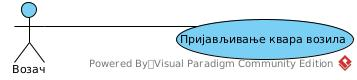
\includegraphics[scale = 0.45]{Slike/SUodrzavanje.jpg}
    \centering
    \caption{Sluchaj upotrebe: Odrz1avanje vozila}
    \label{odrzavanje vozila}
\end{figure}  
Odrz1avanje vozila je sluchaj upotrebe u kom serviser formira bazu podataka vozila, planira i nadgleda popravku, servisiranje i kupovinu vozila. Uchesnici su vozach i serviser. 
\subsubsection{Sluchaj upotrebe: Prijavljivanje kvara vozila}
\begin{itemize}
\item{\textbf{Kratak opis:} Vozach prijavljuje kvar vozila na putu popunjavanjem formulara u okviru sistema. Serviser obradjuje prijavu kvara i shalje povratnu informaciju vozachu preko sitema.}
\item{\textbf{Akteri:} Vozach i serviser}
\item{\textbf{Ulaz:} Podaci o vozilu, prirodi kvara i trenutnoj lokaciji vozacha, podaci o organizaciji popravke kvara }
\item{\textbf{Izlaz:} Poruka o obradi prijave kvara }
\item{\textbf{Preduslovi:} Vozach ima pristup sistemu preko interneta. Serviser ima pristup sistemu. }
\item{\textbf{Postuslovi:} Uspeshno prijavljen kvar.}
\item{\textbf{Glavni tok:} 
\begin{enumerate}
    \item [1.] Vozach pristupa formularu za prijavu kvara u okviru sistema.
    \item[2.] Vozach unosi podatke o vozilu, opis prirode kvara i tachnu lokaciju.
    \item[3.] Klikom na dugme vozach potvrdjuje unete podatke.
    \item[4.] Sistem validira unete podatke.
    \item[5.] Sistem chuva podatke o prijavi kvara.
    \item[6.] Sistem shalje serviseru poruku o prijavljenom kvaru.
    \item[7.] Serviseru se pojavljuje poruka o prijavljenom kvaru.
    \item[8.] Serviser pristupa formularu za obradu prijave kvara.
    \item[9.] Serviser popunjava podatke o organizaciji popravke.
    \item[10.] Klikom na dugme serviser potvrdjuje unos.
    \item[11.] Sistem validira unete podatke.
    \item [12.] Sistem chuva podatke o obradi prijavljenog kvara.
    \item[13.] Sistem shalje poruku vozachu o uspeshno prijavljenom kvaru vozila. 
    \item[14.] Vozachu se prikazuje poruka o uspeshno prijavljenom kvaru.
    
\end{enumerate}

}
\item{\textbf{Alternativni tokovi:} 
\begin{enumerate}
    \item [A1.] \textbf{Neuspeshna validacija unetih podataka o kvaru vozila.} Ukoliko u 4. koraku glavnog toka sistem naidje na neispravno popunjeno polje formulara, sistem c1e markirati isto i obavestiti vozacha. Vozach ispravlja unos. Proces se nastavlja u 3. koraku glavnog toka.
   \item [A2.] \textbf{Neuspeshna validacija unetih podataka o obradi kvara.} Ukoliko u 11. koraku glavnog toka sistem naidje na neispravno popunjeno polje formulara, sistem c1e markirati isto i obavestiti servisera. Serviser ispravlja unos. Proces se nastavlja u 10. koraku glavnog toka.
\end{enumerate}
}
\end{itemize}

\subsubsection{Sluchaj upotrebe: Unoshenje novog vozila u sistem}
\begin{itemize}
\item{\textbf{Kratak opis:} Serviser unosi informacije o vozilu koje u trenutku unosa ne postoji u sistemu. Sistem obradjuje informacije, az1urira se stanje sistema i vrac1a povratna informacija o uspeshnosti unosa.}
\item{\textbf{Akteri:} Serviser}
\item{\textbf{Ulaz:} Podaci o vozilu }
\item{\textbf{Izlaz:} Poruka o uspeshnosti unoshenja vozila u sistem }
\item{\textbf{Preduslovi:} Serviser ima pristup sistemu i poseduje potrebne informacije o novom vozilu. }
\item{\textbf{Postuslovi:} Uspeshno dodato vozilo u sistem.}
\item{\textbf{Glavni tok:} 
\begin{enumerate}
    \item [1.] Serviser pristupa formularu za unos novog vozila u okviru sistema.
    \item[2.] Serviser popunjava traz1ene podatke o vozilu (tehniche podatke, registarski broj tablice, datum isteka registracije, nosivost vozila).
    \item[3.] Serviser potvrdjuje unos podataka klikom na dugme.
    \item[4.] Sistem validira unete podatke.
    \item[5.] Sistem chuva podatke o novom vozilu.
    \item[6.] Prikazuje se poruka o uspeshnosti akcije.
\end{enumerate}

}
\item{\textbf{Alternativni tokovi:} 
\begin{enumerate}
    \item [A1.] \textbf{Neuspeshna validacija unetih podataka.} Ukoliko u 4. koraku glavnog toka sistem naidje na neispravno popunjeno polje formulara, sistem c1e markirati isto i obavestiti servisera. Serviser ispravlja unos. Proces se nastavlja u 3. koraku glavnog toka.
    \item[A2.] \textbf{Odustajanje.} Serviser u 3. koraku klikom na dugme odbacuje unete podatke i odustaje od unoshenja novog vozila u sistem. Informacije o vozilu nisu zapamc1ene u sistemu. Proces se zavrshava.
\end{enumerate}
}
\end{itemize}

\subsubsection{Sluchaj upotrebe: Brisanje postojec1eg vozila iz sistema}

\begin{itemize}
\item{\textbf{Kratak opis:} Serviser brishe postojec1e vozilo iz sistema. Az1urira se stanje sistema i vrac1a povratna informacija o uspeshnosti akcije.}
\item{\textbf{Akteri:} Serviser}
\item{\textbf{Ulaz:} Podaci o vozilu za pretragu }
\item{\textbf{Izlaz:} Poruka o uspeshnosti brisanja vozila iz sistema }
\item{\textbf{Preduslovi:} Serviser ima pristup sistemu i poseduje potrebne informacije o vozilu. Postoje informacije o vozilu u sistemu.}
\item{\textbf{Postuslovi:} Uspeshno obrisano vozilo iz sistema.}
\item{\textbf{Glavni tok:} 
\begin{enumerate}
    \item [1.] Serviser pristupa formularu za brisanje vozila iz sistema.
    \item[2.] Serviser pretraz1uje bazu vozila unoshenjem broja registarske tablice vozila u polje za pretragu.
    \item[3.] Serviser potvrdjuje unos klikom na dugme za pretragu.
    \item[4.] Sistem validira podatke.
    \item[5.] Sistem pronalazi vozilo na osnovu unetih podataka i prikazuje ih.
    \item[6.] Serviser bira jedno od ponudjenih vozila klikom na isto.
    \item[7.] Klikom na dugme serviser shalje zahtev za brisanje sistemu.
    \item[8.] Sistem brishe informacije o vozilu i az1urira bazu vozila.
    \item[9.] Prikazuje se poruka o uspeshnosti izvrshene akcije.
\end{enumerate}

}
\item{\textbf{Alternativni tokovi:} 
\begin{enumerate}
    \item [A1.] \textbf{Neuspeshna validacija podataka za pretragu.} Ukoliko u 4. koraku sistem naidje na neispravno popunjeno polje, obaveshtava servisera adekvatnom porukom. Serviser ispravlja unos i proces se nastavlja u 3. koraku glavnog toka.
    \item[A2.] \textbf{Odustajanje.} Serviser u 7. koraku glavnog toka klikom na dugme odustaje od brisanja vozila. Informacije o vozilu se chuvaju neizmenjene u sistemu. Proces se zavrshava.
\end{enumerate}
}
\end{itemize}

\subsubsection{Sluchaj upotrebe: Az1uriranje postojec1eg vozila u sistemu}

\begin{itemize}
\item{\textbf{Kratak opis:} Serviser menja podatke o postojec1em vozilu sistema. Az1urira se stanje sistema i vrac1a povratna informacija o uspeshnosti akcije.}
\item{\textbf{Akteri:} Serviser}
\item{\textbf{Ulaz:} Novi podaci o vozilu }
\item{\textbf{Izlaz:} Poruka o uspeshnosti izmene podataka o  vozilu }
\item{\textbf{Preduslovi:} Serviser ima pristup sistemu i poseduje potrebne informacije o vozilu. Postoje informacije o vozilu u sistemu.}
\item{\textbf{Postuslovi:} Uspeshno az1urirano vozilo.}
\item{\textbf{Glavni tok:} 
\begin{enumerate}
    \item [1.] Serviser pristupa formularu za az1uriranje vozila.
    \item[2.] Serviser pretraz1uje bazu vozila unoshenjem broja registarske tablice u polje za pretragu.
    \item[3.] Serviser potvrdjuje unos klikom na dugme za pretragu.
    \item[4.] Sistem validira podatke.
    \item[5.] Sistem pronalazi vozila na osnovu unetih podataka i prikazuje ih.
    \item[6.] Serviser bira jedno od ponudjenih vozila klikom na isto.
    \item[7.] Klikom na dugme za az1uriranje prikazuje se formular sa podacima o vozilu koji se trenutno chuvaju u sistemu.
    \item[8.] Serviser unosi nove podatke o vozilu.
    \item[9.] Klikom na dugme serviser potvrdjuje unos.
    \item[10.] Sistem validira podatke.
    \item[11.] Sistem chuva nove podatke o vozilu u bazi.
    \item[12.] Sistem prikazuje poruku o uspeshnosti izmena.
\end{enumerate}

}
\item{\textbf{Alternativni tokovi:} 
\begin{enumerate}
    \item [A1.] \textbf{Neuspeshna validacija podataka za pretragu.} Ukoliko u 4. koraku sistem naidje na neispravno popunjeno polje, obaveshtava servisera adekvatnom porukom. Serviser ispravlja unos i proces se nastavlja u 3. koraku glavnog toka.
    \item [A2.] \textbf{Neuspeshna validacija novih podataka o vozilu} Ukoliko u 10. koraku sistem naidje na neispravno popunjeno polje, markira ga i obaveshtava servisera adekvatnom porukom. Serviser ispravlja unos i proces se nastavlja u 9. koraku glavnog toka.
    \item[A2.] \textbf{Odustajanje.} Serviser u 9. koraku glavnog toka klikom na dugme odustaje od unetih izmena. Chuvaju se se neizmenjeni podaci o vozilu u sistemu. Proces se zavrshava.
\end{enumerate}
}
\end{itemize}


